% Created by tikzDevice version 0.12.3.1 on 2022-09-20 14:26:17
% !TEX encoding = UTF-8 Unicode
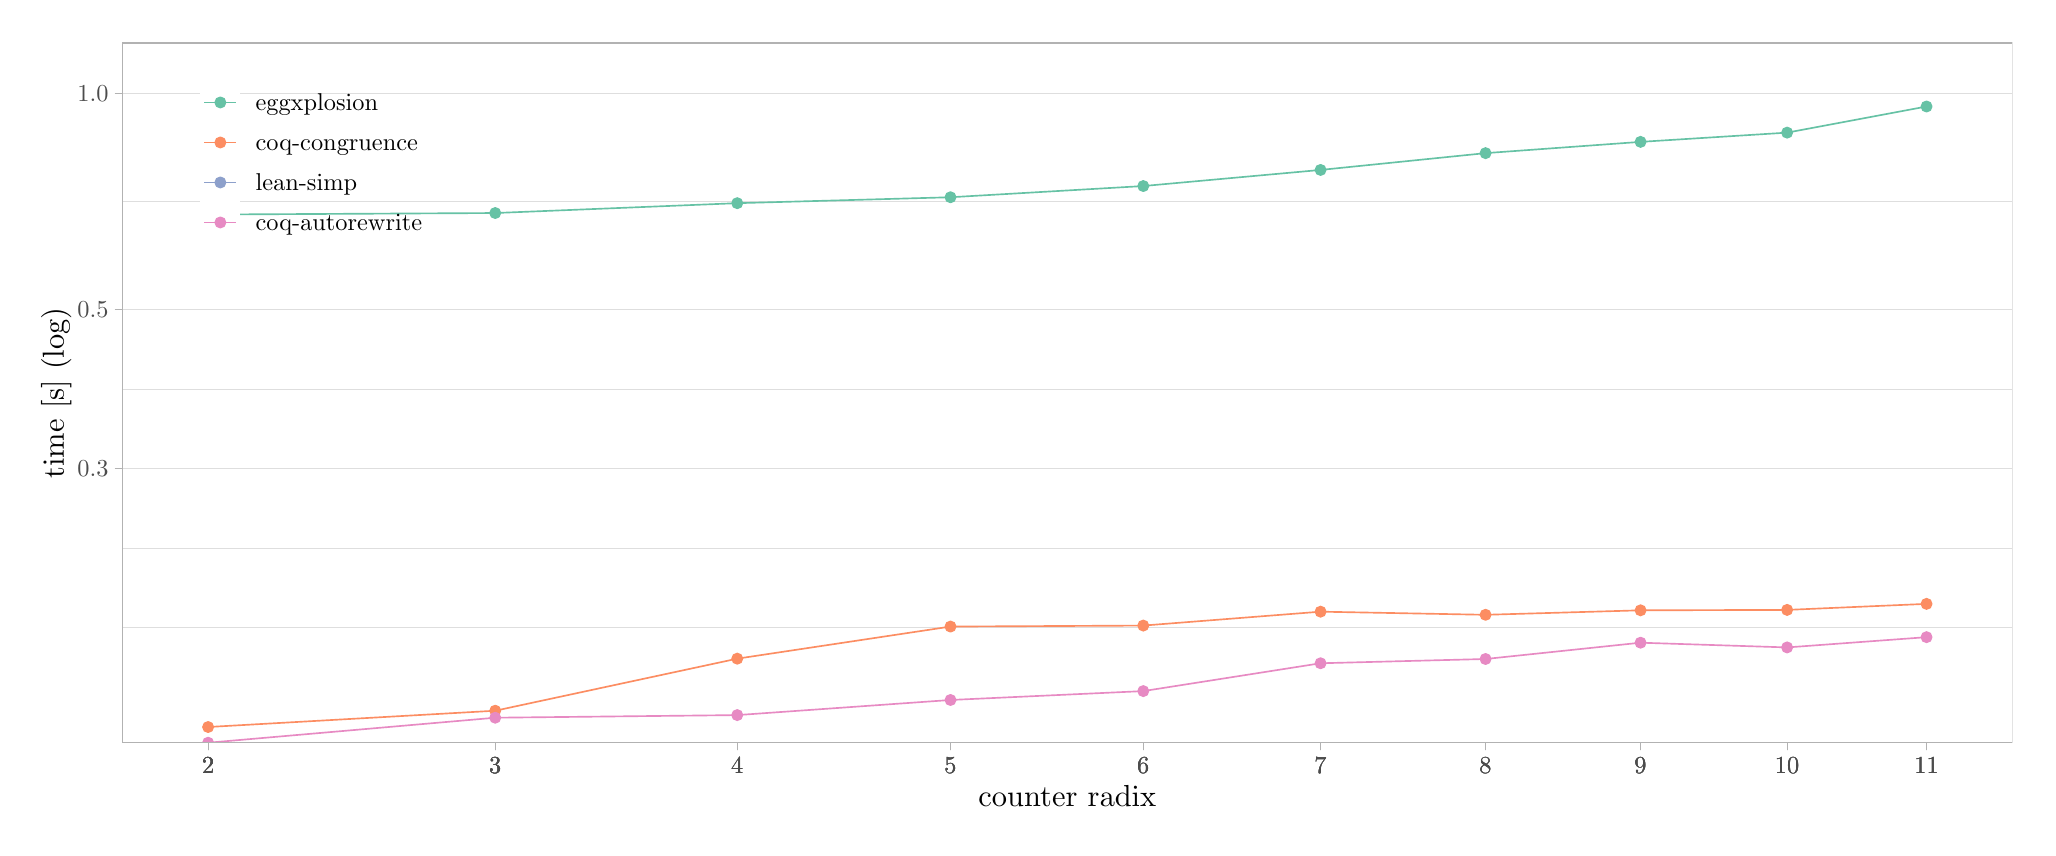
\begin{tikzpicture}[x=1pt,y=1pt]
\definecolor{fillColor}{RGB}{255,255,255}
\path[use as bounding box,fill=fillColor,fill opacity=0.00] (0,0) rectangle (722.70,289.08);
\begin{scope}
\path[clip] (  0.00,  0.00) rectangle (722.70,289.08);
\definecolor{drawColor}{RGB}{255,255,255}
\definecolor{fillColor}{RGB}{255,255,255}

\path[draw=drawColor,line width= 0.6pt,line join=round,line cap=round,fill=fillColor] (  0.00,  0.00) rectangle (722.70,289.08);
\end{scope}
\begin{scope}
\path[clip] ( 34.16, 30.69) rectangle (717.20,283.58);
\definecolor{fillColor}{RGB}{255,255,255}

\path[fill=fillColor] ( 34.16, 30.69) rectangle (717.20,283.58);
\definecolor{drawColor}{gray}{0.87}

\path[draw=drawColor,line width= 0.1pt,line join=round] ( 34.16, 72.39) --
	(717.20, 72.39);

\path[draw=drawColor,line width= 0.1pt,line join=round] ( 34.16,101.13) --
	(717.20,101.13);

\path[draw=drawColor,line width= 0.1pt,line join=round] ( 34.16,158.62) --
	(717.20,158.62);

\path[draw=drawColor,line width= 0.1pt,line join=round] ( 34.16,226.37) --
	(717.20,226.37);

\path[draw=drawColor,line width= 0.3pt,line join=round] ( 34.16,129.88) --
	(717.20,129.88);

\path[draw=drawColor,line width= 0.3pt,line join=round] ( 34.16,187.37) --
	(717.20,187.37);

\path[draw=drawColor,line width= 0.3pt,line join=round] ( 34.16,265.38) --
	(717.20,265.38);
\definecolor{drawColor}{RGB}{102,194,165}
\definecolor{fillColor}{RGB}{102,194,165}

\path[draw=drawColor,line width= 0.4pt,line join=round,line cap=round,fill=fillColor] ( 65.20,221.55) circle (  1.96);
\definecolor{drawColor}{RGB}{141,160,203}
\definecolor{fillColor}{RGB}{141,160,203}

\path[draw=drawColor,line width= 0.4pt,line join=round,line cap=round,fill=fillColor] ( 65.20,214.53) circle (  1.96);
\definecolor{drawColor}{RGB}{252,141,98}
\definecolor{fillColor}{RGB}{252,141,98}

\path[draw=drawColor,line width= 0.4pt,line join=round,line cap=round,fill=fillColor] ( 65.20, 36.37) circle (  1.96);
\definecolor{drawColor}{RGB}{231,138,195}
\definecolor{fillColor}{RGB}{231,138,195}

\path[draw=drawColor,line width= 0.4pt,line join=round,line cap=round,fill=fillColor] ( 65.20, 30.69) circle (  1.96);
\definecolor{drawColor}{RGB}{102,194,165}
\definecolor{fillColor}{RGB}{102,194,165}

\path[draw=drawColor,line width= 0.4pt,line join=round,line cap=round,fill=fillColor] (168.95,222.10) circle (  1.96);
\definecolor{drawColor}{RGB}{252,141,98}
\definecolor{fillColor}{RGB}{252,141,98}

\path[draw=drawColor,line width= 0.4pt,line join=round,line cap=round,fill=fillColor] (168.95, 42.26) circle (  1.96);
\definecolor{drawColor}{RGB}{231,138,195}
\definecolor{fillColor}{RGB}{231,138,195}

\path[draw=drawColor,line width= 0.4pt,line join=round,line cap=round,fill=fillColor] (168.95, 39.73) circle (  1.96);
\definecolor{drawColor}{RGB}{102,194,165}
\definecolor{fillColor}{RGB}{102,194,165}

\path[draw=drawColor,line width= 0.4pt,line join=round,line cap=round,fill=fillColor] (256.40,225.66) circle (  1.96);
\definecolor{drawColor}{RGB}{252,141,98}
\definecolor{fillColor}{RGB}{252,141,98}

\path[draw=drawColor,line width= 0.4pt,line join=round,line cap=round,fill=fillColor] (256.40, 61.07) circle (  1.96);
\definecolor{drawColor}{RGB}{231,138,195}
\definecolor{fillColor}{RGB}{231,138,195}

\path[draw=drawColor,line width= 0.4pt,line join=round,line cap=round,fill=fillColor] (256.40, 40.68) circle (  1.96);
\definecolor{drawColor}{RGB}{102,194,165}
\definecolor{fillColor}{RGB}{102,194,165}

\path[draw=drawColor,line width= 0.4pt,line join=round,line cap=round,fill=fillColor] (333.46,227.80) circle (  1.96);
\definecolor{drawColor}{RGB}{252,141,98}
\definecolor{fillColor}{RGB}{252,141,98}

\path[draw=drawColor,line width= 0.4pt,line join=round,line cap=round,fill=fillColor] (333.46, 72.67) circle (  1.96);
\definecolor{drawColor}{RGB}{231,138,195}
\definecolor{fillColor}{RGB}{231,138,195}

\path[draw=drawColor,line width= 0.4pt,line join=round,line cap=round,fill=fillColor] (333.46, 46.14) circle (  1.96);
\definecolor{drawColor}{RGB}{102,194,165}
\definecolor{fillColor}{RGB}{102,194,165}

\path[draw=drawColor,line width= 0.4pt,line join=round,line cap=round,fill=fillColor] (403.12,231.85) circle (  1.96);
\definecolor{drawColor}{RGB}{252,141,98}
\definecolor{fillColor}{RGB}{252,141,98}

\path[draw=drawColor,line width= 0.4pt,line join=round,line cap=round,fill=fillColor] (403.12, 73.03) circle (  1.96);
\definecolor{drawColor}{RGB}{231,138,195}
\definecolor{fillColor}{RGB}{231,138,195}

\path[draw=drawColor,line width= 0.4pt,line join=round,line cap=round,fill=fillColor] (403.12, 49.35) circle (  1.96);
\definecolor{drawColor}{RGB}{102,194,165}
\definecolor{fillColor}{RGB}{102,194,165}

\path[draw=drawColor,line width= 0.4pt,line join=round,line cap=round,fill=fillColor] (467.18,237.67) circle (  1.96);
\definecolor{drawColor}{RGB}{252,141,98}
\definecolor{fillColor}{RGB}{252,141,98}

\path[draw=drawColor,line width= 0.4pt,line join=round,line cap=round,fill=fillColor] (467.18, 78.05) circle (  1.96);
\definecolor{drawColor}{RGB}{231,138,195}
\definecolor{fillColor}{RGB}{231,138,195}

\path[draw=drawColor,line width= 0.4pt,line join=round,line cap=round,fill=fillColor] (467.18, 59.41) circle (  1.96);
\definecolor{drawColor}{RGB}{102,194,165}
\definecolor{fillColor}{RGB}{102,194,165}

\path[draw=drawColor,line width= 0.4pt,line join=round,line cap=round,fill=fillColor] (526.80,243.74) circle (  1.96);
\definecolor{drawColor}{RGB}{252,141,98}
\definecolor{fillColor}{RGB}{252,141,98}

\path[draw=drawColor,line width= 0.4pt,line join=round,line cap=round,fill=fillColor] (526.80, 76.92) circle (  1.96);
\definecolor{drawColor}{RGB}{231,138,195}
\definecolor{fillColor}{RGB}{231,138,195}

\path[draw=drawColor,line width= 0.4pt,line join=round,line cap=round,fill=fillColor] (526.80, 60.95) circle (  1.96);
\definecolor{drawColor}{RGB}{102,194,165}
\definecolor{fillColor}{RGB}{102,194,165}

\path[draw=drawColor,line width= 0.4pt,line join=round,line cap=round,fill=fillColor] (582.81,247.81) circle (  1.96);
\definecolor{drawColor}{RGB}{252,141,98}
\definecolor{fillColor}{RGB}{252,141,98}

\path[draw=drawColor,line width= 0.4pt,line join=round,line cap=round,fill=fillColor] (582.81, 78.54) circle (  1.96);
\definecolor{drawColor}{RGB}{231,138,195}
\definecolor{fillColor}{RGB}{231,138,195}

\path[draw=drawColor,line width= 0.4pt,line join=round,line cap=round,fill=fillColor] (582.81, 66.84) circle (  1.96);
\definecolor{drawColor}{RGB}{102,194,165}
\definecolor{fillColor}{RGB}{102,194,165}

\path[draw=drawColor,line width= 0.4pt,line join=round,line cap=round,fill=fillColor] (635.77,251.15) circle (  1.96);
\definecolor{drawColor}{RGB}{252,141,98}
\definecolor{fillColor}{RGB}{252,141,98}

\path[draw=drawColor,line width= 0.4pt,line join=round,line cap=round,fill=fillColor] (635.77, 78.69) circle (  1.96);
\definecolor{drawColor}{RGB}{231,138,195}
\definecolor{fillColor}{RGB}{231,138,195}

\path[draw=drawColor,line width= 0.4pt,line join=round,line cap=round,fill=fillColor] (635.77, 65.13) circle (  1.96);
\definecolor{drawColor}{RGB}{102,194,165}
\definecolor{fillColor}{RGB}{102,194,165}

\path[draw=drawColor,line width= 0.4pt,line join=round,line cap=round,fill=fillColor] (686.15,260.59) circle (  1.96);
\definecolor{drawColor}{RGB}{252,141,98}
\definecolor{fillColor}{RGB}{252,141,98}

\path[draw=drawColor,line width= 0.4pt,line join=round,line cap=round,fill=fillColor] (686.15, 80.87) circle (  1.96);
\definecolor{drawColor}{RGB}{231,138,195}
\definecolor{fillColor}{RGB}{231,138,195}

\path[draw=drawColor,line width= 0.4pt,line join=round,line cap=round,fill=fillColor] (686.15, 68.84) circle (  1.96);
\definecolor{drawColor}{RGB}{102,194,165}

\path[draw=drawColor,line width= 0.6pt,line join=round] ( 65.20,221.55) --
	(168.95,222.10) --
	(256.40,225.66) --
	(333.46,227.80) --
	(403.12,231.85) --
	(467.18,237.67) --
	(526.80,243.74) --
	(582.81,247.81) --
	(635.77,251.15) --
	(686.15,260.59);
\definecolor{drawColor}{RGB}{252,141,98}

\path[draw=drawColor,line width= 0.6pt,line join=round] ( 65.20, 36.37) --
	(168.95, 42.26) --
	(256.40, 61.07) --
	(333.46, 72.67) --
	(403.12, 73.03) --
	(467.18, 78.05) --
	(526.80, 76.92) --
	(582.81, 78.54) --
	(635.77, 78.69) --
	(686.15, 80.87);
\definecolor{drawColor}{RGB}{231,138,195}

\path[draw=drawColor,line width= 0.6pt,line join=round] ( 65.20, 30.69) --
	(168.95, 39.73) --
	(256.40, 40.68) --
	(333.46, 46.14) --
	(403.12, 49.35) --
	(467.18, 59.41) --
	(526.80, 60.95) --
	(582.81, 66.84) --
	(635.77, 65.13) --
	(686.15, 68.84);
\definecolor{drawColor}{gray}{0.70}

\path[draw=drawColor,line width= 0.6pt,line join=round,line cap=round] ( 34.16, 30.69) rectangle (717.20,283.58);
\end{scope}
\begin{scope}
\path[clip] (  0.00,  0.00) rectangle (722.70,289.08);
\definecolor{drawColor}{gray}{0.30}

\node[text=drawColor,anchor=base east,inner sep=0pt, outer sep=0pt, scale=  0.88] at ( 29.21,126.85) {0.3};

\node[text=drawColor,anchor=base east,inner sep=0pt, outer sep=0pt, scale=  0.88] at ( 29.21,184.34) {0.5};

\node[text=drawColor,anchor=base east,inner sep=0pt, outer sep=0pt, scale=  0.88] at ( 29.21,262.35) {1.0};
\end{scope}
\begin{scope}
\path[clip] (  0.00,  0.00) rectangle (722.70,289.08);
\definecolor{drawColor}{gray}{0.70}

\path[draw=drawColor,line width= 0.3pt,line join=round] ( 31.41,129.88) --
	( 34.16,129.88);

\path[draw=drawColor,line width= 0.3pt,line join=round] ( 31.41,187.37) --
	( 34.16,187.37);

\path[draw=drawColor,line width= 0.3pt,line join=round] ( 31.41,265.38) --
	( 34.16,265.38);
\end{scope}
\begin{scope}
\path[clip] (  0.00,  0.00) rectangle (722.70,289.08);
\definecolor{drawColor}{gray}{0.70}

\path[draw=drawColor,line width= 0.3pt,line join=round] ( 65.20, 27.94) --
	( 65.20, 30.69);

\path[draw=drawColor,line width= 0.3pt,line join=round] ( 65.20, 27.94) --
	( 65.20, 30.69);

\path[draw=drawColor,line width= 0.3pt,line join=round] ( 65.20, 27.94) --
	( 65.20, 30.69);

\path[draw=drawColor,line width= 0.3pt,line join=round] ( 65.20, 27.94) --
	( 65.20, 30.69);

\path[draw=drawColor,line width= 0.3pt,line join=round] (168.95, 27.94) --
	(168.95, 30.69);

\path[draw=drawColor,line width= 0.3pt,line join=round] (168.95, 27.94) --
	(168.95, 30.69);

\path[draw=drawColor,line width= 0.3pt,line join=round] (168.95, 27.94) --
	(168.95, 30.69);

\path[draw=drawColor,line width= 0.3pt,line join=round] (168.95, 27.94) --
	(168.95, 30.69);

\path[draw=drawColor,line width= 0.3pt,line join=round] (256.40, 27.94) --
	(256.40, 30.69);

\path[draw=drawColor,line width= 0.3pt,line join=round] (256.40, 27.94) --
	(256.40, 30.69);

\path[draw=drawColor,line width= 0.3pt,line join=round] (256.40, 27.94) --
	(256.40, 30.69);

\path[draw=drawColor,line width= 0.3pt,line join=round] (333.46, 27.94) --
	(333.46, 30.69);

\path[draw=drawColor,line width= 0.3pt,line join=round] (333.46, 27.94) --
	(333.46, 30.69);

\path[draw=drawColor,line width= 0.3pt,line join=round] (333.46, 27.94) --
	(333.46, 30.69);

\path[draw=drawColor,line width= 0.3pt,line join=round] (403.12, 27.94) --
	(403.12, 30.69);

\path[draw=drawColor,line width= 0.3pt,line join=round] (403.12, 27.94) --
	(403.12, 30.69);

\path[draw=drawColor,line width= 0.3pt,line join=round] (403.12, 27.94) --
	(403.12, 30.69);

\path[draw=drawColor,line width= 0.3pt,line join=round] (467.18, 27.94) --
	(467.18, 30.69);

\path[draw=drawColor,line width= 0.3pt,line join=round] (467.18, 27.94) --
	(467.18, 30.69);

\path[draw=drawColor,line width= 0.3pt,line join=round] (467.18, 27.94) --
	(467.18, 30.69);

\path[draw=drawColor,line width= 0.3pt,line join=round] (526.80, 27.94) --
	(526.80, 30.69);

\path[draw=drawColor,line width= 0.3pt,line join=round] (526.80, 27.94) --
	(526.80, 30.69);

\path[draw=drawColor,line width= 0.3pt,line join=round] (526.80, 27.94) --
	(526.80, 30.69);

\path[draw=drawColor,line width= 0.3pt,line join=round] (582.81, 27.94) --
	(582.81, 30.69);

\path[draw=drawColor,line width= 0.3pt,line join=round] (582.81, 27.94) --
	(582.81, 30.69);

\path[draw=drawColor,line width= 0.3pt,line join=round] (582.81, 27.94) --
	(582.81, 30.69);

\path[draw=drawColor,line width= 0.3pt,line join=round] (635.77, 27.94) --
	(635.77, 30.69);

\path[draw=drawColor,line width= 0.3pt,line join=round] (635.77, 27.94) --
	(635.77, 30.69);

\path[draw=drawColor,line width= 0.3pt,line join=round] (635.77, 27.94) --
	(635.77, 30.69);

\path[draw=drawColor,line width= 0.3pt,line join=round] (686.15, 27.94) --
	(686.15, 30.69);

\path[draw=drawColor,line width= 0.3pt,line join=round] (686.15, 27.94) --
	(686.15, 30.69);

\path[draw=drawColor,line width= 0.3pt,line join=round] (686.15, 27.94) --
	(686.15, 30.69);
\end{scope}
\begin{scope}
\path[clip] (  0.00,  0.00) rectangle (722.70,289.08);
\definecolor{drawColor}{gray}{0.30}

\node[text=drawColor,anchor=base,inner sep=0pt, outer sep=0pt, scale=  0.88] at ( 65.20, 19.68) {2};

\node[text=drawColor,anchor=base,inner sep=0pt, outer sep=0pt, scale=  0.88] at ( 65.20, 19.68) {2};

\node[text=drawColor,anchor=base,inner sep=0pt, outer sep=0pt, scale=  0.88] at ( 65.20, 19.68) {2};

\node[text=drawColor,anchor=base,inner sep=0pt, outer sep=0pt, scale=  0.88] at ( 65.20, 19.68) {2};

\node[text=drawColor,anchor=base,inner sep=0pt, outer sep=0pt, scale=  0.88] at (168.95, 19.68) {3};

\node[text=drawColor,anchor=base,inner sep=0pt, outer sep=0pt, scale=  0.88] at (168.95, 19.68) {3};

\node[text=drawColor,anchor=base,inner sep=0pt, outer sep=0pt, scale=  0.88] at (168.95, 19.68) {3};

\node[text=drawColor,anchor=base,inner sep=0pt, outer sep=0pt, scale=  0.88] at (168.95, 19.68) {3};

\node[text=drawColor,anchor=base,inner sep=0pt, outer sep=0pt, scale=  0.88] at (256.40, 19.68) {4};

\node[text=drawColor,anchor=base,inner sep=0pt, outer sep=0pt, scale=  0.88] at (256.40, 19.68) {4};

\node[text=drawColor,anchor=base,inner sep=0pt, outer sep=0pt, scale=  0.88] at (256.40, 19.68) {4};

\node[text=drawColor,anchor=base,inner sep=0pt, outer sep=0pt, scale=  0.88] at (333.46, 19.68) {5};

\node[text=drawColor,anchor=base,inner sep=0pt, outer sep=0pt, scale=  0.88] at (333.46, 19.68) {5};

\node[text=drawColor,anchor=base,inner sep=0pt, outer sep=0pt, scale=  0.88] at (333.46, 19.68) {5};

\node[text=drawColor,anchor=base,inner sep=0pt, outer sep=0pt, scale=  0.88] at (403.12, 19.68) {6};

\node[text=drawColor,anchor=base,inner sep=0pt, outer sep=0pt, scale=  0.88] at (403.12, 19.68) {6};

\node[text=drawColor,anchor=base,inner sep=0pt, outer sep=0pt, scale=  0.88] at (403.12, 19.68) {6};

\node[text=drawColor,anchor=base,inner sep=0pt, outer sep=0pt, scale=  0.88] at (467.18, 19.68) {7};

\node[text=drawColor,anchor=base,inner sep=0pt, outer sep=0pt, scale=  0.88] at (467.18, 19.68) {7};

\node[text=drawColor,anchor=base,inner sep=0pt, outer sep=0pt, scale=  0.88] at (467.18, 19.68) {7};

\node[text=drawColor,anchor=base,inner sep=0pt, outer sep=0pt, scale=  0.88] at (526.80, 19.68) {8};

\node[text=drawColor,anchor=base,inner sep=0pt, outer sep=0pt, scale=  0.88] at (526.80, 19.68) {8};

\node[text=drawColor,anchor=base,inner sep=0pt, outer sep=0pt, scale=  0.88] at (526.80, 19.68) {8};

\node[text=drawColor,anchor=base,inner sep=0pt, outer sep=0pt, scale=  0.88] at (582.81, 19.68) {9};

\node[text=drawColor,anchor=base,inner sep=0pt, outer sep=0pt, scale=  0.88] at (582.81, 19.68) {9};

\node[text=drawColor,anchor=base,inner sep=0pt, outer sep=0pt, scale=  0.88] at (582.81, 19.68) {9};

\node[text=drawColor,anchor=base,inner sep=0pt, outer sep=0pt, scale=  0.88] at (635.77, 19.68) {10};

\node[text=drawColor,anchor=base,inner sep=0pt, outer sep=0pt, scale=  0.88] at (635.77, 19.68) {10};

\node[text=drawColor,anchor=base,inner sep=0pt, outer sep=0pt, scale=  0.88] at (635.77, 19.68) {10};

\node[text=drawColor,anchor=base,inner sep=0pt, outer sep=0pt, scale=  0.88] at (686.15, 19.68) {11};

\node[text=drawColor,anchor=base,inner sep=0pt, outer sep=0pt, scale=  0.88] at (686.15, 19.68) {11};

\node[text=drawColor,anchor=base,inner sep=0pt, outer sep=0pt, scale=  0.88] at (686.15, 19.68) {11};
\end{scope}
\begin{scope}
\path[clip] (  0.00,  0.00) rectangle (722.70,289.08);
\definecolor{drawColor}{RGB}{0,0,0}

\node[text=drawColor,anchor=base,inner sep=0pt, outer sep=0pt, scale=  1.10] at (375.68,  7.64) {counter radix};
\end{scope}
\begin{scope}
\path[clip] (  0.00,  0.00) rectangle (722.70,289.08);
\definecolor{drawColor}{RGB}{0,0,0}

\node[text=drawColor,rotate= 90.00,anchor=base,inner sep=0pt, outer sep=0pt, scale=  1.10] at ( 13.08,157.13) {time [s] (log)};
\end{scope}
\begin{scope}
\path[clip] (  0.00,  0.00) rectangle (722.70,289.08);
\definecolor{fillColor}{RGB}{255,255,255}

\path[fill=fillColor] ( 62.40,254.82) rectangle ( 76.85,269.27);
\end{scope}
\begin{scope}
\path[clip] (  0.00,  0.00) rectangle (722.70,289.08);
\definecolor{drawColor}{RGB}{102,194,165}
\definecolor{fillColor}{RGB}{102,194,165}

\path[draw=drawColor,line width= 0.4pt,line join=round,line cap=round,fill=fillColor] ( 69.63,262.05) circle (  1.96);
\end{scope}
\begin{scope}
\path[clip] (  0.00,  0.00) rectangle (722.70,289.08);
\definecolor{drawColor}{RGB}{102,194,165}

\path[draw=drawColor,line width= 0.6pt,line join=round] ( 63.84,262.05) -- ( 75.41,262.05);
\end{scope}
\begin{scope}
\path[clip] (  0.00,  0.00) rectangle (722.70,289.08);
\definecolor{fillColor}{RGB}{255,255,255}

\path[fill=fillColor] ( 62.40,240.37) rectangle ( 76.85,254.82);
\end{scope}
\begin{scope}
\path[clip] (  0.00,  0.00) rectangle (722.70,289.08);
\definecolor{drawColor}{RGB}{252,141,98}
\definecolor{fillColor}{RGB}{252,141,98}

\path[draw=drawColor,line width= 0.4pt,line join=round,line cap=round,fill=fillColor] ( 69.63,247.59) circle (  1.96);
\end{scope}
\begin{scope}
\path[clip] (  0.00,  0.00) rectangle (722.70,289.08);
\definecolor{drawColor}{RGB}{252,141,98}

\path[draw=drawColor,line width= 0.6pt,line join=round] ( 63.84,247.59) -- ( 75.41,247.59);
\end{scope}
\begin{scope}
\path[clip] (  0.00,  0.00) rectangle (722.70,289.08);
\definecolor{fillColor}{RGB}{255,255,255}

\path[fill=fillColor] ( 62.40,225.91) rectangle ( 76.85,240.37);
\end{scope}
\begin{scope}
\path[clip] (  0.00,  0.00) rectangle (722.70,289.08);
\definecolor{drawColor}{RGB}{141,160,203}
\definecolor{fillColor}{RGB}{141,160,203}

\path[draw=drawColor,line width= 0.4pt,line join=round,line cap=round,fill=fillColor] ( 69.63,233.14) circle (  1.96);
\end{scope}
\begin{scope}
\path[clip] (  0.00,  0.00) rectangle (722.70,289.08);
\definecolor{drawColor}{RGB}{141,160,203}

\path[draw=drawColor,line width= 0.6pt,line join=round] ( 63.84,233.14) -- ( 75.41,233.14);
\end{scope}
\begin{scope}
\path[clip] (  0.00,  0.00) rectangle (722.70,289.08);
\definecolor{fillColor}{RGB}{255,255,255}

\path[fill=fillColor] ( 62.40,211.46) rectangle ( 76.85,225.91);
\end{scope}
\begin{scope}
\path[clip] (  0.00,  0.00) rectangle (722.70,289.08);
\definecolor{drawColor}{RGB}{231,138,195}
\definecolor{fillColor}{RGB}{231,138,195}

\path[draw=drawColor,line width= 0.4pt,line join=round,line cap=round,fill=fillColor] ( 69.63,218.69) circle (  1.96);
\end{scope}
\begin{scope}
\path[clip] (  0.00,  0.00) rectangle (722.70,289.08);
\definecolor{drawColor}{RGB}{231,138,195}

\path[draw=drawColor,line width= 0.6pt,line join=round] ( 63.84,218.69) -- ( 75.41,218.69);
\end{scope}
\begin{scope}
\path[clip] (  0.00,  0.00) rectangle (722.70,289.08);
\definecolor{drawColor}{RGB}{0,0,0}

\node[text=drawColor,anchor=base west,inner sep=0pt, outer sep=0pt, scale=  0.88] at ( 82.35,259.02) {eggxplosion};
\end{scope}
\begin{scope}
\path[clip] (  0.00,  0.00) rectangle (722.70,289.08);
\definecolor{drawColor}{RGB}{0,0,0}

\node[text=drawColor,anchor=base west,inner sep=0pt, outer sep=0pt, scale=  0.88] at ( 82.35,244.56) {coq-congruence};
\end{scope}
\begin{scope}
\path[clip] (  0.00,  0.00) rectangle (722.70,289.08);
\definecolor{drawColor}{RGB}{0,0,0}

\node[text=drawColor,anchor=base west,inner sep=0pt, outer sep=0pt, scale=  0.88] at ( 82.35,230.11) {lean-simp};
\end{scope}
\begin{scope}
\path[clip] (  0.00,  0.00) rectangle (722.70,289.08);
\definecolor{drawColor}{RGB}{0,0,0}

\node[text=drawColor,anchor=base west,inner sep=0pt, outer sep=0pt, scale=  0.88] at ( 82.35,215.66) {coq-autorewrite};
\end{scope}
\end{tikzpicture}
